%%%%%%%%%%%%%%%%%%%%%%%%%%%%%%%%%%%%%%%%%%%%%%%%%%%%%%%%%%%%%%%%%%%%%%%%%%%%%%%%
%2345678901234567890123456789012345678901234567890123456789012345678901234567890
%        1         2         3         4         5         6         7         8

%\documentclass[letterpaper, 10 pt, conference]{ieeeconf}  % Comment this line out
                                                          % if you need a4paper
\documentclass[a4paper, 10pt, conference]{ieeeconf}      % Use this line for a4
                                                          % paper

\IEEEoverridecommandlockouts                              % This command is only
                                                          % needed if you want to
                                                          % use the \thanks command
\usepackage{epsf,graphicx}
\usepackage{latexsym,amssymb}
\usepackage{setspace,cite}
\usepackage{etoolbox}

\overrideIEEEmargins
% See the \addtolength command later in the file to balance the column lengths
% on the last page of the document

\title{\LARGE \bf
Object Flow
}

\author{
Juan Manuel Perez Rua, Tomas Crivelli and Patrick Perez% <-this % stops a space
\thanks{This was supported by Technicolor R\&D}
\thanks{Juan Manuel Perez Rua  is with Technicolor R\&D,
        {\tt\small juanmanuel.perezrua@technicolor.com}}%
\thanks{Tomas Crivelli  is with Technicolor R\&D,
        {\tt\small tomas.crivelli@technicolor.com}}%
\thanks{Patrick Perez  is with Technicolor R\&D,
        {\tt\small patrick.perez@technicolor.com}}%
}
\begin{document}



\maketitle
\thispagestyle{empty}
\pagestyle{empty}


%===========================================================
\begin{abstract}

Superpixels and over segmentation techniques
became a widely used pre-processing stage for a
large number of machine vision applications, after the
original concept was introduced \cite{c1}. Superpixels are
traditionally used as performance booster for several
other techniques. However, it is still mostly related to
single frame processing \cite{c1}\cite{c10}\cite{c11}. In the search for
consistency in superpixel labeling through video,
some authors have proposed different techniques,
which go from simple extension to supervoxels\cite{c9}\cite{c11},
to more complicated approaches \cite{c8}. These
approaches, nonetheless, usually require a global
processing and knowledge of all (or several of) the
video frames beforehand. In this paper we propose a superpixel
matching technique which assumes a flowlike
behavior in the image sequences (natural video), and
propose an application for improving object segmentation in videos.

\end{abstract}
\section{Introduction}
\label{sec:introduction}

Object tracking and optical flow are two of the main components in the
computer vision toolbox, and have been focus of great research efforts, 
leading to significant progress in the last years \cite{c16,c17}. 
The object tracking problem in videos consists on estimating the 
position of a target in every frame, given an initial position. On the
other hand, the optical flow between a pair of frames consists on finding a displacement vector 
for each pixel of the first image, namely a {\it dense motion  or displacement field}. Even though for several
applications a complete (i.e. for every pixel) motion-field is needed, other applications like
human-computer interaction, object editing in video or structure-from-motion,
may only focus on an interest object and thus, only a subset of motion vectors is required. 
In such scenarios combining optical flow and object tracking in a unified 
framework appears useful and the precision of the object motion description 
could be enhanced. For instance, even with modern optical flow approaches, 
the long term dense motion estimation remains a challenge \cite{c20,c22}.  At large, object trackers provide a more robust, 
longer term motion estimation featuring a global description of an object, specially after recent works based on tracking-by-detection approaches \cite{c16,c23,c24}. 
On the other side, they lack the (sub) pixel precision of dense optical flow estimators, as well as a deeper use of contextual information for bundle motion 
vector estimation. 
Even more,  object trackers and optical flow give precious hints for other fundamental tools such as 
object segmentation in video. Nevertheless,
these two techniques were not deeply studied in the literature as a unified problem. Though optical flow has been widely used as a motion 
feature for object tracking \cite{c25}, feeding a dense motion estimator with tracking information is not being fully exploited.
This being said, we introduce  a new problem which we call object flow. Thus, for a given object of interest, 
the object flow is the set of displacement vectors for every pixel that belong to the target in a first frame, 
towards another frame of the sequence. In other words, a dense displacement  field constrained to the spatial support of the object. 
Note that by definition this induces a segmentation of the target and of the motion field.

We can define more precisely the object flow by starting with an image sequence, say $I_t, t:0..N-1$, and an initial 
position of the interest object in the first frame of this sequence. Let $\mathcal{R} \in \Omega$ be the region corresponding to the support of the object in the
bi-dimensional grid $\Omega$. Then, the object flow, $\mathcal{O}(x)$,  is defined as $\mathcal{O}(x) = d_{0,t}(x), \forall x \in \mathcal{R}$.

A straightforward solution to this problem would be to compute the optical flow field between a pair of frames, and to apply 
a segmentation mask to recover the desired motion vectors. Nevertheless, this approach carries several 
problems. For example, a globally computed optical flow method can affect small objects motion, because of 
the common use of heavy regularization prior. Moreover, finding the pixels that belong to the interest object in several frames is a difficult problem. 
We propose an approach to reduce these problems.

%The present paper is organized as follows. We describe our pipeline for object flow, including the novel concept of superpixel flow
%in Sec. \ref{sec:desc} and its use in object segmentation in videos. In following
%sections some results showing how 
%the object flow overpass state of the art optical flow methods for object motion flows 
%estimation are discussed. Finally, some insights and conclusions are given.


\section{Algorithm description}
\label{sec:desc}

The Fig. \ref{figurelabel_sys} shows a simplified block diagram of the proposed system. Two details are important, 
the use of the tracker window to initialize a segmentation procedure, and the use of this segmentation over the tracked window 
to perform a more precise motion flow computation in the interest pixels. The dotted line represents the possible interaction 
between precise flow information with the next tracker state. For instance, the current object flow can work as direction hint, and 
the segmentation information can be used to improve the sampling process of the learning stage in several trackers by detection methods \cite{c22}, and 
thus the tracker and motion flow algorithm can work for mutual enhancement.

   \begin{figure}[thpb]
      \centering
      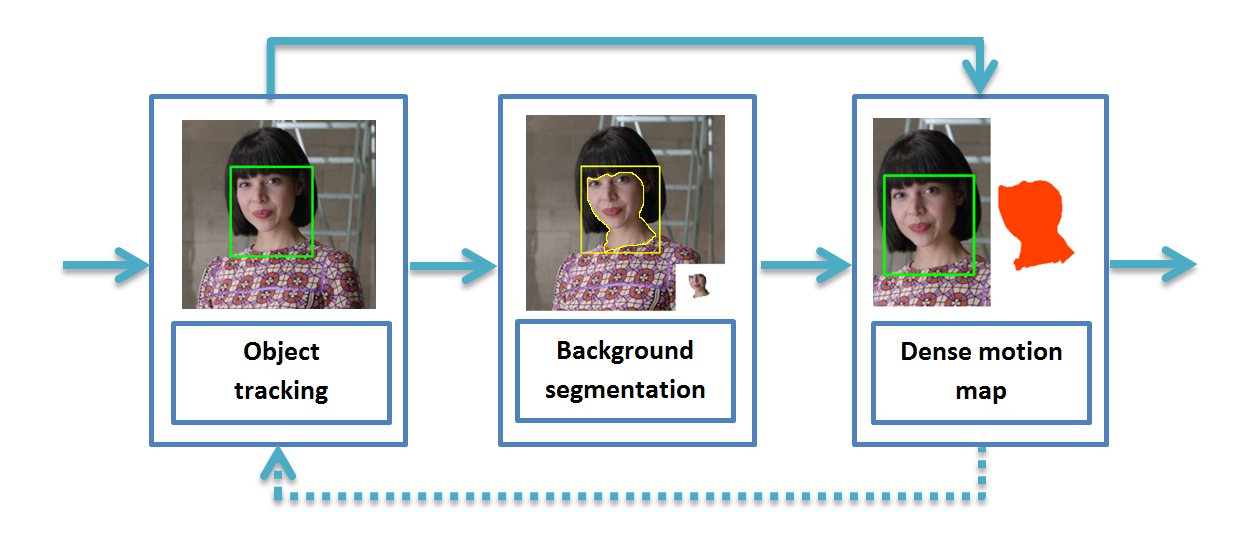
\includegraphics[width=1.00\textwidth]{../images/system.png}
      \caption{Block diagram of the proposed pipeline.}
      \label{figurelabel_sys}
   \end{figure}

The first step in the object flow pipeline can be selected according to specific need for a given application. We prefer, in general, tracking-by-detection methods 
like $Struck$ \cite{c22} or $MIL$ \cite{c23}, but other approaches could be followed. In the second place, for the object segmentation in video we propose the use 
of labelled background regions through the concept of superpixel flow, which is explained in the next section. Finally, the flow motion field is computed within the segmentation boundaries and long term dense 
point trajectories may be extracted from this.


\subsection{Superpixel flow}
\label{sec:suppix}

%\subsection{Problem definition}
%Superpixels and over segmentation techniques became a widely used pre-processing
 %stage for a large number of machine vision applications, after the
%original concept was introduced \cite{c1}. Superpixels are traditionally used as 
%performance booster for several other techniques. However, it is still mostly related to
%single frame processing \cite{c1}\cite{c10}\cite{c11}. In the search for
%consistency in superpixel labeling through video, some authors have proposed different 
%techniques, which go from simple extension to supervoxels\cite{c9}\cite{c11},
%to more complicated approaches \cite{c8}. These approaches, nonetheless, usually require a 
%global processing and knowledge of all (or several of) the video frames beforehand. 

As a preprocessing step in the object flow pipeline, we propose a superpixel matching technique which assumes a flowlike behavior in the image 
sequences (natural video), which can be used to track superpixels. 
%Some previous work have been done towards a
%superpixel based image comparison using the Earth Mover's Distance, by taking superpixels 
%as bins of a global histogram \cite{c2}. The label propagation or superpixel flow can be
%achieved with this technique as a byproduct, by selecting the superpixel in the second frame that 
%maximize the flow from each superpixel in the first frame.
%By taking into account superpixels computed separately in images, so the video process can be 
%performed with only two frames at a time, we move towards a more time efficient approach. 
This matching, however, has to comply with a set of constraints. 
Firstly, two correspondent superpixels should be similar in terms of some appearance
feature, which most likely depends on the way the superpixelization was performed (color, texture,
shape). Also, the superpixel flow  should maintain certain global regularity (at least for
superpixels that belong to the same object). %In this sense, it seems
%natural that the problem of superpixel flow could be solved with a discrete energy minimization
%procedure. 
If the size compactness of the superpixels is maintained,  it actually seems to 
share some of the properties of the optical flow problem, with the difference that the
smoothness is usually a very strong constraint for the last one. 
The strength of this smoothness prior relies not only in the nature of the problem, but also
because it gives better cues towards an easier-to-minimize global approach.

The objective of the superpixel flow is therefore to find the best labeling $l$ for every superpixel $p$
(with $l_p \in {0,1,...N-1}$) between a pair of frames ($I_{0}$,$I_{1}$), but holding a flow-like behaviour.

Thus, the superpixelization should maintain certain size homogeneity within a single frame. Some super
pixel techniques can cope with this requirement \cite{c9}\cite{c10}. For the experiments presented 
in this work, we prefer the SLIC method \cite{c9}, which usually gives
good results in terms of size homogeneity and compactness of the superpixelization. 
%The proposed steps to solve the propagation problem assume this requirement is hold. 
%For other kind of the techniques, other approaches should be followed.

%\addtolength{\textheight}{-3cm}   % This command serves to balance the column lengths
%%%%%%%%%%%%%%%%%%%%%%%%%%%%%%%%%%%%%%%%%%%%%%%%%%%%%%%%%%%%%%%%%%%%%%%%%%%%%%%%

%\subsection{Energy Formulation}

Inspired by a large number of optical flow and stereo techniques \cite{c7}\cite{c12}\cite{c13}, 
the superpixel flow can be modelled with pairwise Markov Random Fields. If
%the matching is performed with MAP inference, its posterior probability is: 
the matching is performed with MAP inference, its energy function extracted from the posterior probability is: 
%\begin{equation}
%P(l|I_0,I_1) = \displaystyle \prod_{p \in \Omega} \mathrm{e}^{-D_p(l_p;I_0,I_1)} 
%\prod_{p,q \in \mathcal{N}} \mathrm{e}^{-S_{p,q}(L_p;L_q)} 
%\label{eq_prob}
%\end{equation}

%With $l$ the set of labels of the super pixels in $I_0$,
%that match with those in $I_1$.
%$ \mathcal{N}_p $ is a neighborhood of the
%superpixel $p$, which defines its adjacency. Given this posterior probability,
%the equivalent energy function can be directly obtained
%by extracting the negative logarithm of the posterior,

\begin{equation}
E(l) = \displaystyle \sum_{p \in \Omega} D_p(L_p;I_0,I_1) +
\sum_{p,q \in \mathcal{N}} S_{p,q}(L_p,L_q)
\label{eq_energy}
\end{equation}

With $l$ the set of labels of the super pixels in $I_0$,
that match with those in $I_1$.
$ \mathcal{N} $ is a neighbourhood of the
superpixel $p$, which defines its adjacency. Given this posterior probability,
the equivalent energy function can be directly obtained
by extracting the negative logarithm of the posterior,

The terms $D$, and $S$ in (\ref{eq_energy}) stand for data term and spatial smoothness terms as they
are popularly known in the MRF literature. The first one determines how accurate is the labeling in terms
of consistency of the measured data (color, shape,etc.). In the classical optical flow formulation of this equation,
the data term corresponds to the pixel brightness conservation\cite{c7}\cite{c5}. However, as superpixels are a set
of similar (or somehow homogeneous) pixels, an adequate color based feature can be a low dimensional
color histogram. So $D$ can be written more precisely as the Hellinger distance between the histograms:

\begin{equation}
D_p(l_p;I_0,I_1) = \sqrt{ 1 - \frac{1}{\sqrt{\bar{h}(p)\bar{h}(p')N^2} } \sum_{i}\sqrt{h_{i}(p)h_{i}(p')} }
\label{eq_Dp}
\end{equation}

Where $h(p)$ and $h(p')$ are the histograms of the superpixel $p$ and its correspondent superpixel in the
second frame $I_1$. %The function $\rho$ is the Bhattacharyya distance. 
Note that the low dimensional histogram gives certain robustness against noise,
and slowly changing colors between frames. 

In the other hand, the spatial term is a penalty function for horizontal
and vertical changes of the vectors that have origin in the centroid of the superpixel of the first frame and
end in the centroid of the superpixel of the second frame.

\begin{equation}
S_{p,q}(l_p, l_q) = \lambda(p)
  \sqrt{\frac{|u_{p_c}-u_{q_c}|}{\|p_c-q_c\|}+ \frac{|v_{p_c}-v_{q_c}|}{\|p_c-q_c\|}}
\label{eq_Spq}
\end{equation}
\begin{center}
 where, $ \lambda(p) = (1 + \rho(h(p),h(q)))^2 $ \\
\end{center}

In (\ref{eq_Spq}) the operator $\rho$ is the Hellinger distance as used in the
data term (\ref{eq_Dp}). The histogram distance is nonetheless computed between superpixels $p$ and $q$, 
which belong to the same neighbourhood. The superpixels centroids are noted as $q_c$ and $p_c$, 
and $u$ and $v$ are the horizontal and vertical changes between centroids.
This term is usual in the MRF formulation and has a smoothing effect in superpixels that belong to the
same object. It has to be observed that when two close superpixels are different, thus, more probable to
belong to different objects within the image, the term $\lambda$ allows them to have
matches that do not hold the smoothness prior with the same strength. 
It has to be noted that the proposed energy function is highly non-convex.

%\subsection{Energy Minimization}

%A fair amount of work has been dedicated to discrete optimization techniques in computer vision,
%leading to well-defined and widely tested approaches to solve pairwise MRF\cite{c3}\cite{c4}.
%However, some of the approaches restrict the construction of the spatial term, and/or enforce
%limitations in the number of labels \cite{c3}.
%Because of the high amount of possible labels for  each superpixel in the proposed approach, the use of the
%Fusion Moves \cite{c7} technique seems to be well suited.
%This algorithm employs the Quadratic Pseudo-Boolean Optimization (QPBO), to combine
%incremental sets of proposal labelings, resulting in a semi-globally-optimal solution \cite{c4}.
%Thus, the minimization starts by proposing a set of possible solutions, and iteratively merges them with
%the QPBO technique. \\
%The candidate solutions depend on the problem to be solved. 
%For example, in stereo superpixel matching, some assumptions related to the cameras 
%layout can be made to generate solutions.
The Quadratic Pseudo-Boolean Optimization (QPBO) \cite{c3}\cite{c4} is used to minimize the proposed energy function, 
by merging a set of candidate matches for every superpixel in the first frame.
%In a more generic sense, other assumptions can be made towards candidate generation. 
For instance, for a given superpixel in the initial frame, the corresponding 
matching would be the most similar one in terms of color, shape, or the spatial distance. More candidate solutions can be added by defining a
neighbourhood in the second frame and select random pairs from every neighbourhood of every superpixel
in the first frame. %This is more suitable for problems where the images are extracted from the same video
%sequence. 
%To speed-up the minimization procedure, the QBPO properties can be exploted. For instance, the fusion of the
%proposed solutions is always guaranteed of lowest or equal energy than the two proposals. Thus, one could
%split the fusion procedure in several cores and build a hierarchichal chain as fusions of proposal are subsequently fused.

%   \begin{figure}[thpb]
%      \centering
%      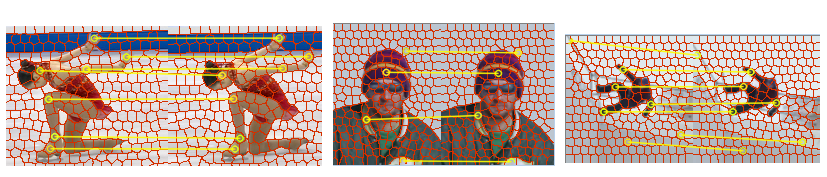
\includegraphics[width=1.00\textwidth]{images/matches.png}
%      \caption{The yellow lines show selected superpixel
%		matching between pairs of consecutive frames in a video
%		with the proposed method. The video frames go from right
%		to left.}
%      \label{figurelabel_matches}
%   \end{figure}

%\subsection{Matching results}

\ifcsdef{r@accv_format}{
   \begin{figure}[thpb]
      \centering
      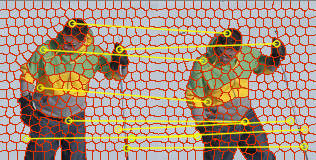
\includegraphics[width=0.70\textwidth]{../images/matches_snowshoes.png}
      \caption{The yellow lines show selected superpixel
		matching between a pair of distant frames in the Snow Shoes sequence.}
      \label{figurelabel_matchessnow}
   \end{figure}   
	\setlength{\belowcaptionskip}{-10pt}
}{
   \begin{figure}[thpb]
      \centering
      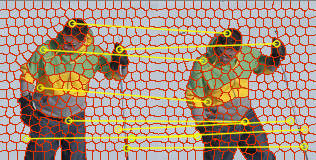
\includegraphics[width=0.5\textwidth]{../images/matches_snowshoes.png}
      \caption{The yellow lines show selected superpixel
		matching between a pair of distant frames in the Snow Shoes sequence.}
      \label{figurelabel_matchessnow}
   \end{figure}   
	\setlength{\belowcaptionskip}{-10pt}
}

%The Fig. \ref{figurelabel_matches} shows some examples of superpixel matching with the presented method. 
%It can be seen that the matching performs well even in difficult cases, like the hands in the top row. It has to be noted
%as well that even in superpixels where there is a lack of texture, there is correct matching. This seems to be
%the effect of enforcing the regularization between superpixels that are close, but are also similar to
%each other.
 
% Moreover, unlike most of the optical flow methods, superpixel flow extends 
 %naturally for more distant frames. 
The Fig. \ref{figurelabel_matchessnow} shows
 results for large separations between frames. % without tweaking or adjusting any parameters. 
For this case, however, the matches in the textureless part of the scene
 are mostly invalids. Though this is expected because of the aperture problem and
 heavy occlusions.

%%%%%%%%%%%%%%%%%%%%%%%%%%%%%%%%%%%%%%%%%%%%%%%%%%%%%%%%%%%%%%%%%%%%%%%%%%%
% Juan Manuel Perez Rua
%%%%%%%%%%%%%%%%%%%%%%%%%%%%%%%%%%%%%%%%%%%%%%%%%%%%%%%%%%%%%%%%%%%%%%%%%%%

\section{Background regions tracking and segmentation}
\label{sec:segm}
The algorithm proposed in \cite{c18}, offers a good deal in terms of
background-foreground separation from user interaction. A technique like this, however,
performs very well in still images, but it may not be well adapted for sequential videos. 
Extensions to this method, like the GrabCut algorithm \cite{c14}, work by implementing an iterative graph-cut based 
minimization to separate regions according to appearance information from a loosely drawn rectangle around the object, and small user-interaction-based hints. 
Given the tracker state for every frame, the minimization procedure of the methods in \cite{c18} and \cite{c14} could be extended to video. However, 
a lot of details in the segmentation contour may be lose if no fine hints are given.
These hints usually depend on on-the-fly supervised methods. However, this need could be minimized in videos, given the extra information that offers the dynamics of the sequence.
Some authors had approached the graph-cut based segmentation techniques in sequential
videos to propagate a consistent segmentation \cite{c15}. However, some more work on reducing user interaction given the extra flow-like information
that video sequences offer is still needed.
Determining the spatial support of the object in a given frame benefits from the output of the tracker. Appearance cues alone, learned inside and outside the tracking window 
can result in a misleading modelling of the foreground and the background. In contrast, we propose to perform foreground-background segmentation by tracking 
background pixels surrounding the target, thanks to the tracker output. Thus, the pixels that are initially outside the tracker window, 
are followed through the sequence and as long as they enter the tracked region, they can be safely labelled as background. 
This idea can be observed in the Fig.  \ref{figurelabel_entering}, 
where the object window given by the tracker (green) loosely separates the foreground from the background. Points outside the tracker (blue) are labelled as background in previous frames, and as they enter the tracker window (red points), they can be used to improve the modelling  of the foreground and the background. 
The red window is used to save computational power by avoiding to track points that are too far from the interest object.

   \begin{figure}[thpb]
      \centering
      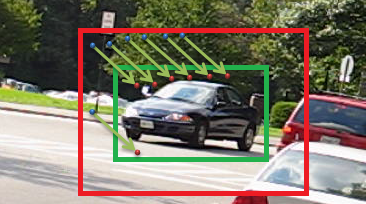
\includegraphics[height=0.285\textheight]{../images/tracking_points.png}
      \caption{Example image of points entering a tracking region (green) due to object motion in a video sequence.}
      \label{figurelabel_entering}
   \end{figure}
\setlength{\belowcaptionskip}{-10pt}

   \begin{figure}[thpb]
      \centering
      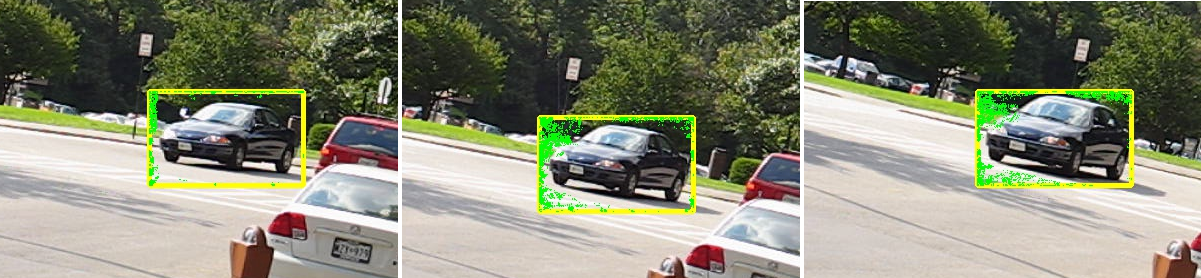
\includegraphics[width=1\textwidth]{../images/pointTr.png}
      \caption{Point tracking using an optical flow method.}
      \label{pointtr}
   \end{figure}


This idea can be applied in several levels in a video sequence. The first method to develop such an algorithm is to do it in the pixel level. The Fig. \ref{pointtr} shows some results by applying 
a dense optical flow technique (Fast Block Matching) in an external window. However, as it can appreciated, the results are rather sparse and after some time, the regularization of the 
optical flow method leads to some of the points being wrongly tracked inside the object boundaries. Both problems, sparsity and tracking errors due to drift and regularization, can be 
overcome by implementing the same idea, but in the superpixel level.
To save computational power, the tracked superpixels are 
limited to the ones that fall inside a control region (red box in the Fig.  \ref{figurelabel_entering}). 

Normally, after several frames, 
the labelled superpixels will almost completely cover the unwanted areas in a dynamic scene. We call this process background segments tracking and the process is summarized in the 
Algorithm \ref{algo1}.  The Fig. \ref{figurelabel_spflow} shows this idea in a real scenario. From left to right, initially the superpixels with 
elements outside the bounding box are labelled as background (green), then, as the sequence changes, the labelled superpixels flow inside the window, giving hints for the model initialization in the background-foreground separation algorithm.

\begin{algorithm}[ht]
\caption{Background regions tracking between a frames A and B}
\label{algo1}
\begin{algorithmic}
\REQUIRE list: $superpixelsA, superpixelsB$, rect: $trackerA, trackerB$, vector: $prev\_labels$

\STATE vector: $new\_labels$
\STATE $computeSuperPixelFlow()$
\FORALL{$superpixel \in superpixelsA$}
    \STATE $matches[superpixel] = getMatchesFromFlow(superpixel)$

	\COMMENT{ Check is previously labelled superpixels fall inside $trackerB$ }
	\IF{$superpixel \in prev\_labels$}
		\STATE $matchAB = superpixelsB[ matches[superpixel] ]$
    		\IF{$matchAB \in trackerB$} 
    			\STATE $new\_labels.push\_back( matchAB )$
    		\ENDIF
	\ENDIF 

	\COMMENT{ Check is new labelled superpixels fall inside $trackerB$ }    
    \IF{$superpixel \notin trackerA$} 
    	    \STATE $matchAB = superpixelsB[ matches[superpixel] ]$
    		\IF{$matchAB \in trackerB$} 
    			\STATE $new\_labels.push\_back( matchAB )$
    		\ENDIF
    	\ENDIF
\ENDFOR

\RETURN $new\_labels$
\end{algorithmic}
\end{algorithm}

At this point, some generic segmentation technique can be connected to the pipeline to refine the segmentation (e.g. region growing). However, graph based segmentation methods are preferred (\cite{c18}\cite{c15}) because the usual user interaction can be replaced by the tracked background regions, and the algorithms are faster and more robust.

   \begin{figure}[thpb]
      \centering
      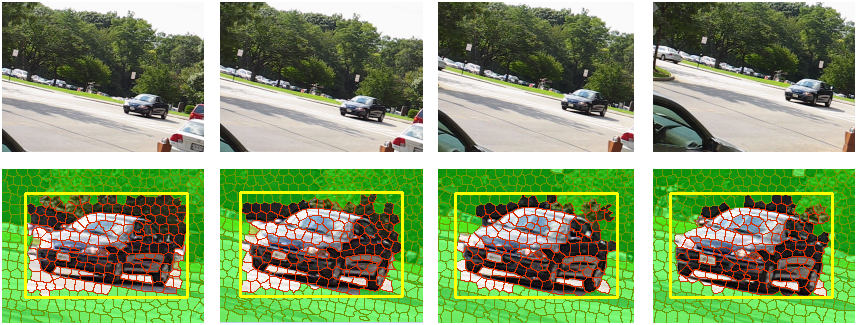
\includegraphics[width=1\textwidth]{../images/suppixflow2.png}
      \caption{Background segments automatic labelling and propagation, the flow goes from left to right.}
      \label{figurelabel_spflow}
   \end{figure}

\subsection{Segmentation results}

Fig. \ref{figurelabel_walking} shows the results for an image sequence where the interest object is the head of a person.
The head tracker and the superpixel flow provide information for better background-foreground separation. The
background-foreground models are updated as the frames go on, giving more robustness for sequential
propagation of the segmentation. The method is tested in the Walking Couple sequence, by allowing only a small amount of iterations in the
graph based segmentation. Observe how the contour in the man's head is correctly delineated when
another person's head occludes part of it. In this case, the superpixels that belong to the woman’s face
were correctly propagated and thus, labelled as background. Its also impressive that the segmentation process recovers after a heavy occlusion.
In this case, the fact that the tracker is also robust to the occlusion is a key factor that help the system maintain a correct segmentation through such a difficult 
case.

   \begin{figure}[thpb]
      \centering
      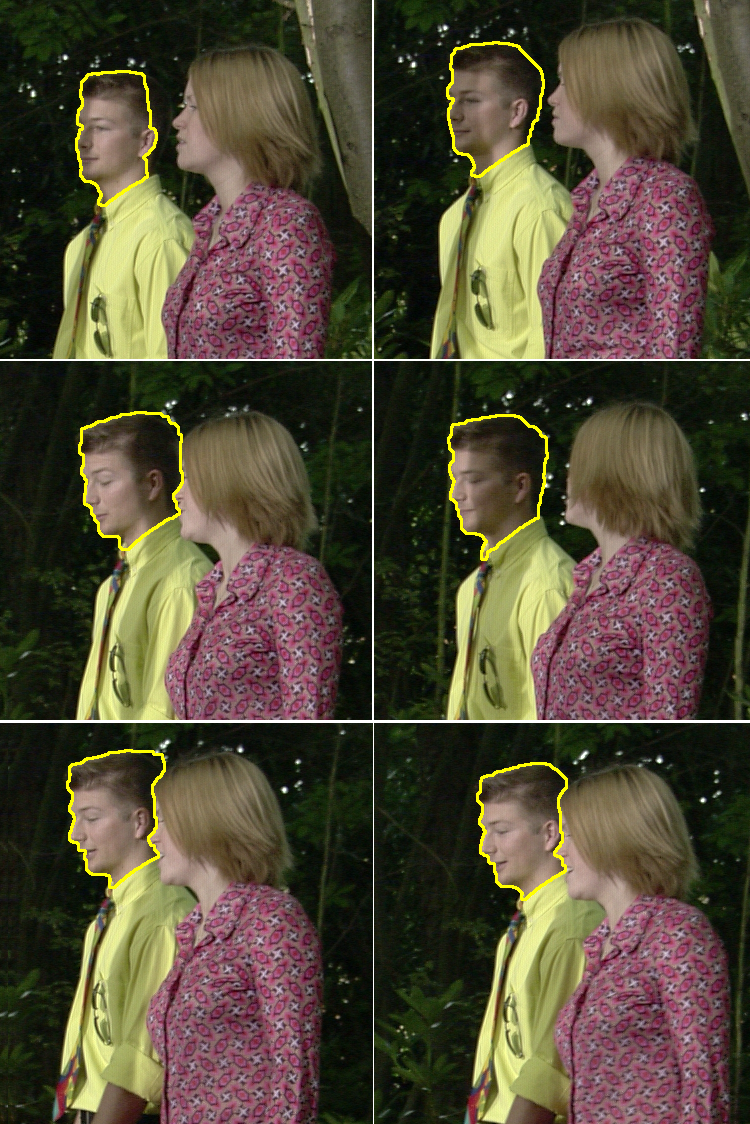
\includegraphics[width=1.0\textwidth]{../images/Sequence.png}
      \caption{Segmentation through the sequence “Walking
	       Couple” (Yellow contour) initialized in the man’s head. The yellow box correspond to the tracker output.
	        The labelled background superpixel are not shown for clarity.}
      \label{figurelabel_walking}
   \end{figure}

In order to understand the effect of including superpixel propagation in a video sequence for object
segmentation, some results are shown in the Fig. \ref{figurelabel_comp}. For these experiments only one iteration is
allowed in the graph-cut based methods. The top row frames (Fig. \ref{figurelabel_comp}) were initialized only with the tracker, 
and the bottom row was initialized with the superpixel tracking technique. 
Observe that in general, the contour delineated is usually better in terms of precision and
stability for the later one. Complete segmentation results can be observed in the Appendix \ref{app:seg}.

   \begin{figure}[thp]
      \centering
      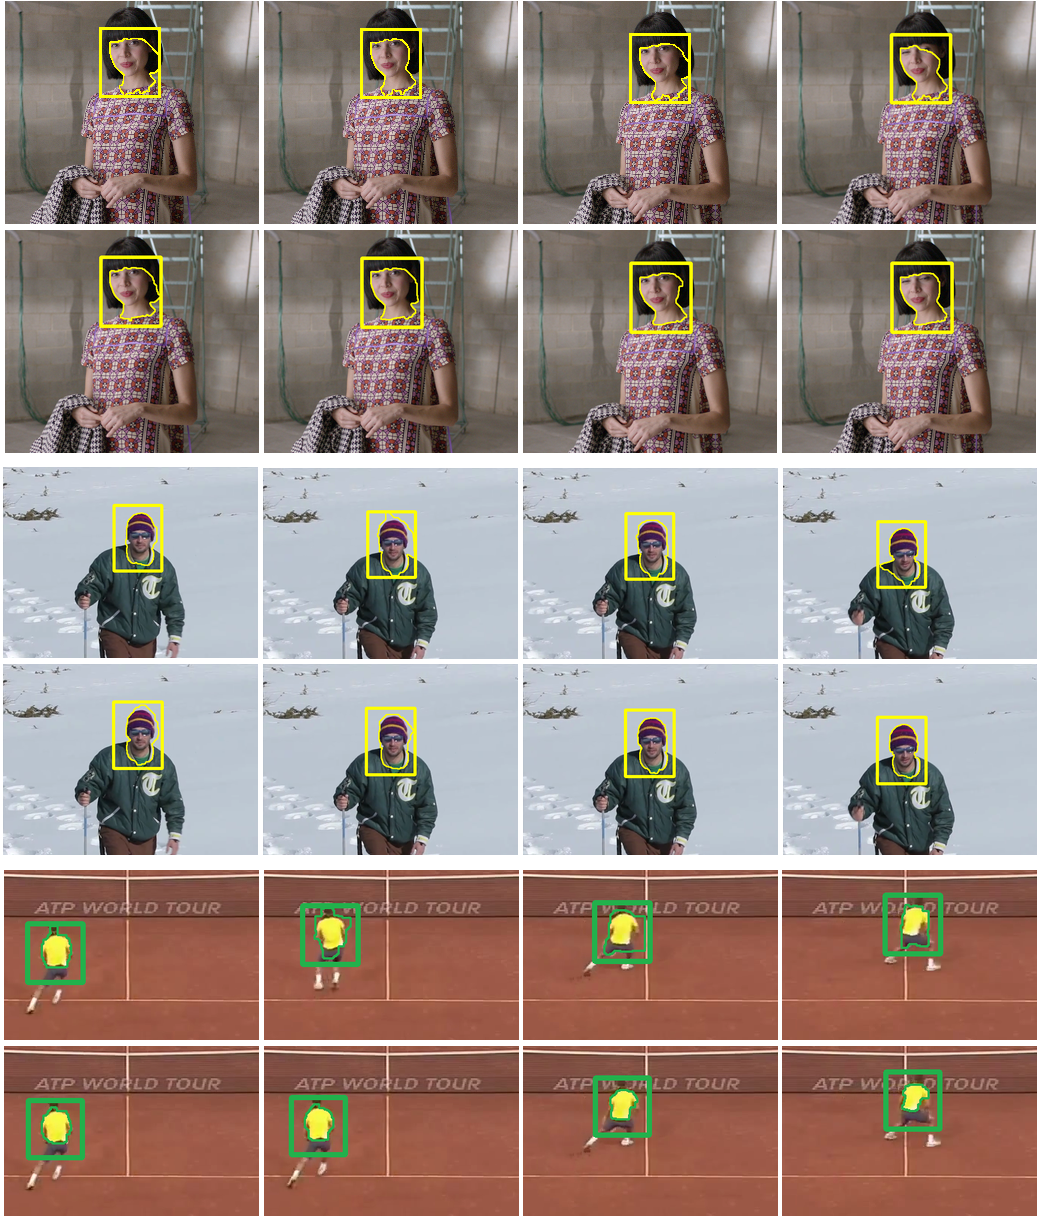
\includegraphics[width=1.0\textwidth]{../images/compareSegm.png}
      \caption{Face segmentation in the “Amelie Retro” and the
	      “Snow shoes” sequences in several different frames, and T-shirt extraction from Tennis sequence. For each
	       group, the Top Row: One-iteration window-based graph-cuts;
	       and the Bottom Row: One-iteration graph-cuts initialized with superpixel tracking.}
      \label{figurelabel_comp}
   \end{figure}

\section{Flow estimation}
%\subsection{Flow estimation}
\label{sec:core}

The object flow consist on computing the motion field for an object of interest through an image
sequence. The most usual approach to solve a problem like this is to implement some of the available
optical flow techniques through the complete sequence and perform the flow integration. 
However, this process results in high levels of motion drift \cite{c18}\cite{c19} and usually the motion of the interest
object is affected by a global regularization. In some extreme cases, the interest object motion
may be totally blurred and other techniques have to be incorporated. Moreover, the diversity
of natural video sequences makes difficult the choice of one optical flow technique over another, even when specialized
databases are at hand \cite{c17}, because currently no single method can achieve a strong 
performance in every of the available datasets. Most of these methods consist in the minimization 
of an energy function with two terms (As was previously mentioned in the Sec. \ref{chap:intro}). The data
term is mostly shared between different approaches, but the prior or spatial term is different, and basically states 
under what conditions the optical flow smoothness should be maintained or not. In a global approach, however,
this is a difficult concept to define. Most of these smoothness terms rely in appearance differences or gradients.
All these meaning that, unavoidably, some methods may be more reliable for some cases but weaker for others. 
It can be argued that this behaviour may be caused because most of the techniques do not count with a way to identify 
firmly where exactly this smoothness prior can be applied. 

It is difficult, nevertheless, to blame the authors for the choice of some regularization 
terms, since the more robust the regularization terms is, and the higher level knowledge is applied, the more difficult is to minimize the 
energy function, and thus, the more difficult is to obtain a reliable global solution. 
The modern advances in non-convex optimization methods have allowed some authors 
to go further in the writing of these energy functions, but at the end they still rely in the pixel level to determine whether a strong regularization 
should be applied to a zone or not.


   \begin{figure}[thpb]
      \centering
      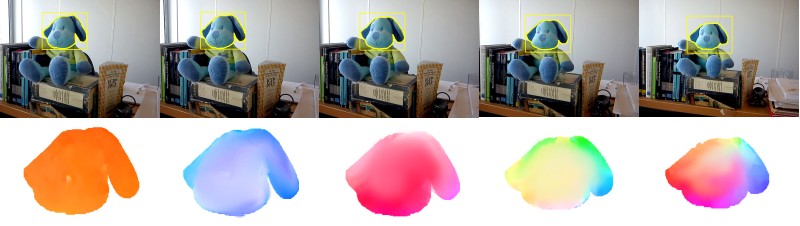
\includegraphics[width=1.0\textwidth]{../images/objectflow.png}
      \caption{Object flow with the color code of \cite{c17} (bottom) for frames in the Puppy sequence (up). }
      \label{of}
   \end{figure}

The main idea behind the object flow is that given the availability of several robust tracking techniques, and the proposed
segmentation method for video, the optical flow computation can be refined by computing it successively between pairs
of tracked windows. The basic proposal to perform this refinement consist on considering the segmentation limits  as reliable smoothness boundaries. 
This is, of course, under the assumption that the motion is indeed smooth within the object region. 
This is assumption is not far from reality in most scenes with an interest object, and it is indeed a better way to determine the limits of the regularization 
than using the difference between raw pixel values.
Naturally, as the object tracker is included, is expected that the object flow should be more robust to rapid motions than the
optical flow. 
Thus, the full motion is split in two, the long range motion, given by the tracker window, and the precision part, given by the targeted optical flow. The Fig. \ref{of} shows 
the object flow for a frame in the Puppy sequence. Observe the motion vectors are computed only inside the object of interest, preserving a strong smoothing prior, but 
also allowing internal variations in the flow. 

As a first approximation to the object flow, the Simple Flow technique \cite{c21} is taken as core base. This is because of its scalability 
to higher resolutions and because its specialization to the concept of object flow is only natural. The reason behind this is that in the Simple Flow pipeline 
the smoothness localization can be easily specified through computation masks. More specifically, the initial computation mask is derived from 
the segmentation performed as prior step. An iterative multi-scale approach based on this initialization follows. The original method uses bilateral filtering to refine each flow result. 
However, as a reliable segmentation mask is provided, this bilateral filtering is replaced by a Gaussian filter applied within the limits of this mask, highly improving the speed of the 
flow estimation. 

   \begin{figure}[thpb]
      \centering
      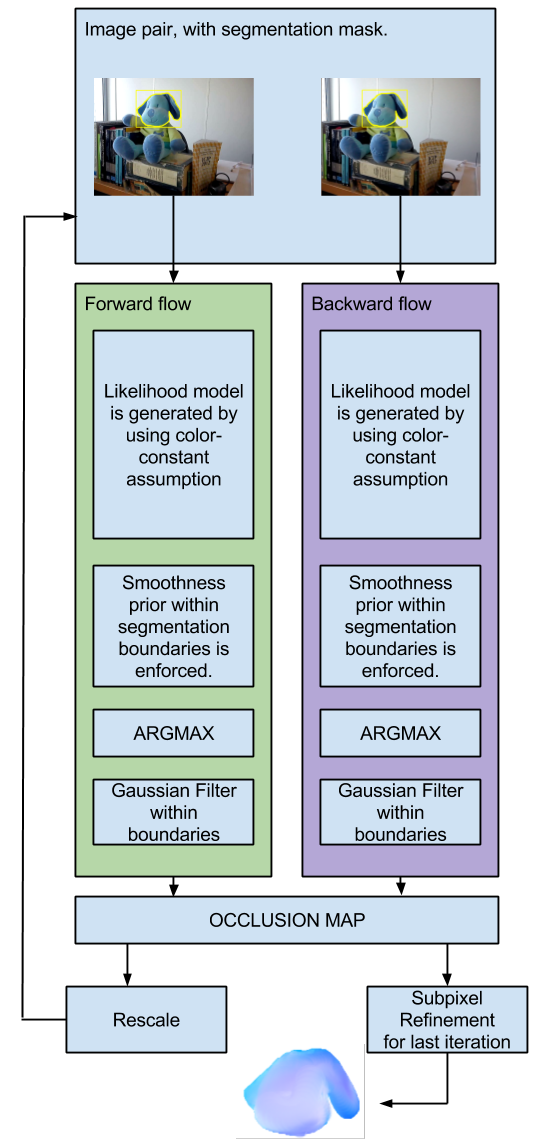
\includegraphics[height=1.0\textheight]{../images/simpleobjectflow.png}
      \caption{ Simple object flow algorithm diagram.}
      \label{sof_d}
   \end{figure}

In more detail, 
for every pixel within the segmentation boundaries a vector $e$ of dimension $n^2$ is computed 
by extracting a color difference $n$x$n$ window centred in that pixel. The energy $E$ (as in \ref{eq_simple}) is computed 
within the 
segmentation boundaries 
by applying a bilateral filter, 
using the color data of the initial 
frame to define the filter weights. 
The flow for the given pixel is the vector that minimizes $E$. The final bilateral filter applied over the computed flow field for every scale is replaced by a Gaussian filter limited by the segmentation masks. The process is done twice, from $I_t$ to $I_{t+1}$ and vice-versa. 
An occlusion mask is generated by eliminating the flows that do not correspond with its 
backward counterpart ($||(u_f,v_f)-(-u_b,-v_b)||$ is too high). The process is repeated in 
several scales to account for possible large motions inside the studied object (Fig. \ref{sof_d}).

However, direct modifications in other optical flow methods can be further studied. For instance, in graph-cut based 
minimization approaches, the regularity constraints can be precisely targeted by disconnecting foreground pixels from background ones.

   \begin{figure}[thpb]
      \centering
      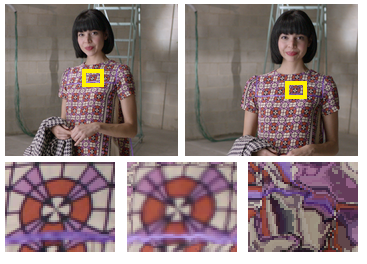
\includegraphics[width=0.66\textwidth]{../images/objectflow_nosegm.png}
      \caption{Top row: First and last frames used from the Amelia sequence. Bottom row: From left to right: Groundtruth patch; patch generated with the 
basic object flow combining the {\it Struck} Tracker and the {\it TVL1} optical flow; and patch generated with the globally computed  {\it TVL1} optical flow.}
      \label{of_nose}
   \end{figure}

The object flow concept is valid, however, for those cases where there is not a separable object, and the segmentation is not valid or possible to extract. 
In order to show this and the fact that only combining the tracker information with a locally computed optical flow is already an improvement to a global 
optical flow, the Fig. \ref{of_nose} shows an experiment where a patch from a dress is extrapolated by using the most basic object flow definition (no segmentation) 
and by a globally computed optical flow. It can be seen that the results are better for the first method.




\section{Conclusions}

A framework to combine tracking and optical flow methods to improve 
object based dense motion description is presented. The pipeline is 
composed of three main steps, object tracking, segmentation and 
flow estimation. For the segmentation step a new promising video object 
segmentation algorithm was proposed, and, to the best of our knowledge, 
the introduced superpixel flow is the first energy based algorithm for superpixel matching.
For the last step, we presented a flow estimation method based on a modification of the simple-flow method to use 
the obtained segmentation mask. The experiments showed that this object based flow estimation improves the dense motion 
estimation for an object in comparisson to optical flow techniques.
Future work includes to explore the use of the object flow as feedback hint for tracking-by-detection methods. 
Furthermore, the use of other optical flow techniques as base of the object flow is a matter of great interest as more precise methods could be found.
Finally, several kind of applications of the object flow can be more deeply approached. For instance, 
in the structure-from-motion pipeline, video editing and video inpainting, among others.



%A method for superpixel matching in a flow-like
%behavior had been presented. We may call it superpixel propagation, or super-pixel flow. This
%technique shows robustness in the labeling of the
%matches, and seems to be able to improve the results
%for object segmentation in video sequences when
%using the Grab-cut algorithm. Another motivation for
%this technique, however may be as initialization of
%optical flow techniques, to obtain more robust results
%due to a good initial guess for energy minimization
%methods. This has to be looked at more deeply in future work.
%===========================================================
\bibliographystyle{splncs}
\begin{thebibliography}{99}

\bibitem{c1}
J. Malik and X. Ren, Learning a classification model for segmentation, {\it Computer Vision, International Conference}, 2003.

\bibitem{c2}
S. Boltz; F. Nielsen and S. Soatto, Earth mover distance on superpixels, {\it International Conference on Image Processing}, 2010.

\bibitem{c3}
E. Boros; P. Hammer and G. Tavares, Preprocessing of unconstrained quadratic binary optimization, {\it RUTCOR}, 2010.

\bibitem{c4}
E. Boros and P. Hammer, Pseudo-boolean optimization, {\it Discrete applied Mathematics.}, 2002.

\bibitem{c5}
B. Horn and B. Schunck, Determining Optical Flow, {\it Artificial Intelligence}, 1981.

\bibitem{c6}
H. Ishikawa and P. Bouthemy, Multimodal estimation of discontinous optical flow using Markov random fields, {\it TPAMI.}, 1993.

\bibitem{c7}
V. Lempitsky, S. Roth and C. Rother, Fusion Flow: Discrete-Continuos optimization for optical flow estimation, {\it Computer Vision and Pattern Recognition}, 2008.

\bibitem{c8}
M. Reso and J. Jachalsky, Temporally Consistent Superpixels, {\it International Conference Computer Vision.}, 2011.

\bibitem{c9}
R. Achanta; A. Shaji; K. Smith; Aurelien Lucchi; P. Fua and S. Susstrunk, SLIC Superpixels compared to state of the art superpixel methods, {\it Discrete applied Mathematics.}, 2002.

\bibitem{c10}
F. Perbet and A. Maki, Homogeneus superpixels from random walks, {\it MVA.}, 2011.

\bibitem{c11}
C. Xu and J.J. Corso. Evaluation of super-voxel methods for early video proccesing, {\it Computer Vision and Pattern Recognition}. 2012.

\bibitem{c12}
A. Shekhovtsov, I. Kovtun and V. Hlavac. Efficient MRF deformation model for non-rigid image matching, {\it Computer Vision and Pattern Recognition}. 2007.

\bibitem{c13}
J. Sun, N.N Shen and H.Y. Shum. Stereo matching using propagation belief, {\it TPAMI}. 2003.

\bibitem{c14}
C. Rother, V. Kolmogorov and A. Blake. Grabcut: Interactive foreground extraction using iterated graph cuts, {\it SIGGRAPH}. 2004.

\bibitem{c15}
L. Yang, Y. Guo, X. Wu and X. Wang. A new video segmentation approach: Grabcut in local window,  {\it Soft Computing and Pattern Recognition}. 2011.

\bibitem{c16}
Y. Wu, J. Lim and M.-H. Yang. Online object tracking: A benchmark, {\it Computer Vision and Pattern Recognition}. 2013.

\bibitem{c17}
S. Baker, D. Scharstein, J.P. Lewis, S. Roth, M.J. Black and R. Szeliski. A Database and Evaluation Methodology for Optical Flow, {\it International Journal Computer Vision}. 2013.

\bibitem{c18}
Y. Boykov, M-P. Jolly. Interactive Graph Cuts for Optimal Boundary \& Region Segmentation of Objects in N-D images, {\it International Conference on Computer Vision}. 2013.

\bibitem{c19}
W. Li, D. Cosker and M. Brown. An anchor patch based optimization framework for reducing optical flow drift in long image sequences, {\it Asian Conference on Computer Vision}. 2012.

\bibitem{c20}
T. Crivelli, P.-H. Conze, P. Robert, M. Fradet and P. Perez. Multi-step flow fusion: towards accurate and dense correpondence in long video shots, {\it British Conference Machine Vision}. 2012.

\bibitem{c21}
M. Tao, J. Bai, P. Kohli, and S. Paris. SimpleFlow: A Non-iterative, Sublinear Optical Flow Algorithm, {\it Computer Graphics Forum, Eurographics}. 2012.

\bibitem{c22}
Brox, A. Bruhn, N. Papenberg, J. Weickert. High accuracy optical flow estimation based on a theory for warping. {\it European Conference in Computer Vision}. 2004.

\bibitem{c23}
S. Hare, A. Saffari, and P.H.S. Torr, Struck: Structured Output Tracking with Kernels.  {\it International Conference on Computer Vision}. 2011.

\bibitem{c24}
B. Babenko, M.H. Yang, and S. Belongie. Visual Tracking with Online Multiple Instance Learning. {\it Computer Vision and Pattern Recognition}. 2009.

\bibitem{c25}
J. Shi and C. Tomasi. Good features to track. {\it Conference on Computer Vision and Pattern Recognition }, 1994. 


\end{thebibliography}
%===========================================================

\end{document}
